\begin{tikzpicture}[x=1cm, y=1cm, font=\sffamily\footnotesize,
  ptitle/.style={anchor=west, font=\sffamily\bfseries\small, text=narrareddeep},
  textbox/.style={draw=phaseA!60, fill=phaseA!6, rounded corners=2pt, inner sep=4pt, anchor=north west,
                  align=left, font=\sffamily\scriptsize},
  lbl/.style={draw=#1, fill=white, fill opacity=0.9, text opacity=1, rounded corners=1pt, inner sep=1.6pt,
              line width=0.6pt, font=\sffamily\scriptsize},
  lblkey/.style={draw=#1, fill=white, fill opacity=0.95, text opacity=1, rounded corners=1pt, inner sep=1.8pt,
                 line width=1.0pt, font=\sffamily\scriptsize\bfseries},
  lead/.style={draw=#1, line width=0.7pt},
  path/.style={-{Latex[length=2.6mm, width=2.4mm]}, draw=black!85, line width=1.6pt},
  imgcap/.style={anchor=north, font=\sffamily\scriptsize, text=black!60},
  chip/.style={draw=black!30, fill=white, rounded corners=6pt, inner sep=2.5pt, font=\sffamily\footnotesize},
  flow/.style={-{Latex[length=1.6mm]}, draw=black!50, line width=0.6pt},
  lab/.style={anchor=east, font=\sffamily\footnotesize, text=black!75},
  txt/.style={anchor=west, font=\sffamily\footnotesize, text=black!75}]

\node[ptitle] at (0,0.000) {(a) The task and its room (AI2-THOR rendering of the benchmark trial)};
\node[textbox, text width=14.70cm] (obs) at (0,-0.280) {\textbf{Goal.} Your task is to: put a mug in desk.\\[1pt]\textbf{Initial observation.} You are in the middle of a room. Looking quickly around you, you see a bed 1, a desk 2, a desk 1, a drawer 6, a drawer 5, a drawer 4, a drawer 3, a drawer 2, a drawer 1, a garbagecan 1, a laundryhamper 1, a safe 1, a shelf 6, a shelf 5, a shelf 4, a shelf 3, a shelf 2, and a shelf 1.};
\begin{scope}[shift={($(obs.south west)+(0,-0.25)$)}]
\node[anchor=north west, inner sep=0] at (0.000,0.000) {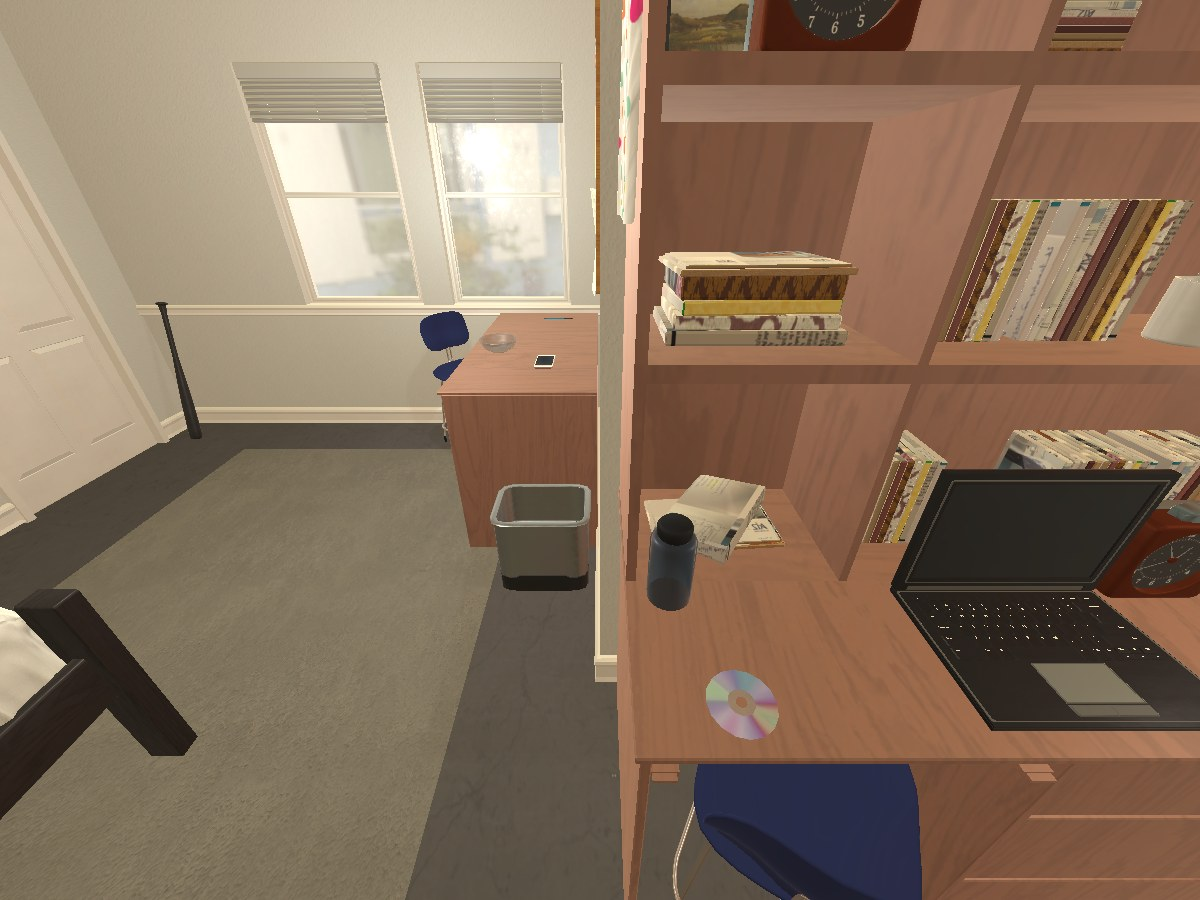
\includegraphics[width=8.508cm]{figures/cases/task0_view1.jpg}};
\draw[black!35, line width=0.4pt] (0.000,0.000) rectangle ++(8.508,-6.381);
\draw[dimF, line width=1.1pt] (8.295,-2.216) circle (0.302);
\draw[lead=dimF] (8.295,-2.216) -- (8.064,-1.754);
\fill[dimF] (8.295,-2.216) circle (0.06);
\node[lblkey=dimF] at (8.064,-1.754) {mug};
\draw[liftpositive, line width=1.1pt, rounded corners=1pt] (3.098,-2.226) rectangle (4.233,-3.878);
\draw[lead=liftpositive] (3.666,-3.052) -- (3.666,-2.552);
\fill[liftpositive] (3.666,-3.052) circle (0.06);
\node[lblkey=liftpositive] at (3.666,-2.552) {desk: put it here};
\draw[dimA, line width=1.1pt, rounded corners=1pt] (6.587,-0.624) rectangle (8.501,-2.581);
\draw[lead=dimA] (7.544,-1.602) -- (6.491,-1.249);
\fill[dimA] (7.544,-1.602) circle (0.06);
\node[lblkey=dimA] at (6.491,-1.249) {shelf: the mug is here};
\fill[black!55] (6.438,-4.931) circle (0.06);
\node[lbl=black!45] at (6.438,-4.931) {desk};
\draw[lead=black!55] (5.906,-1.602) -- (5.006,-1.794);
\fill[black!55] (5.906,-1.602) circle (0.06);
\node[lbl=black!45] at (5.006,-1.794) {shelves};
\fill[black!55] (0.698,-4.999) circle (0.06);
\node[lbl=black!45] at (0.698,-4.999) {bed};
\draw[lead=black!55] (7.675,-6.005) -- (7.675,-5.505);
\fill[black!55] (7.675,-6.005) circle (0.06);
\node[lbl=black!45] at (7.675,-5.505) {drawers};
\draw[lead=black!55] (3.829,-3.815) -- (3.829,-3.315);
\fill[black!55] (3.829,-3.815) circle (0.06);
\node[lbl=black!45] at (3.829,-3.315) {garbagecan};
\node[anchor=north west, inner sep=0] at (8.758,0.000) {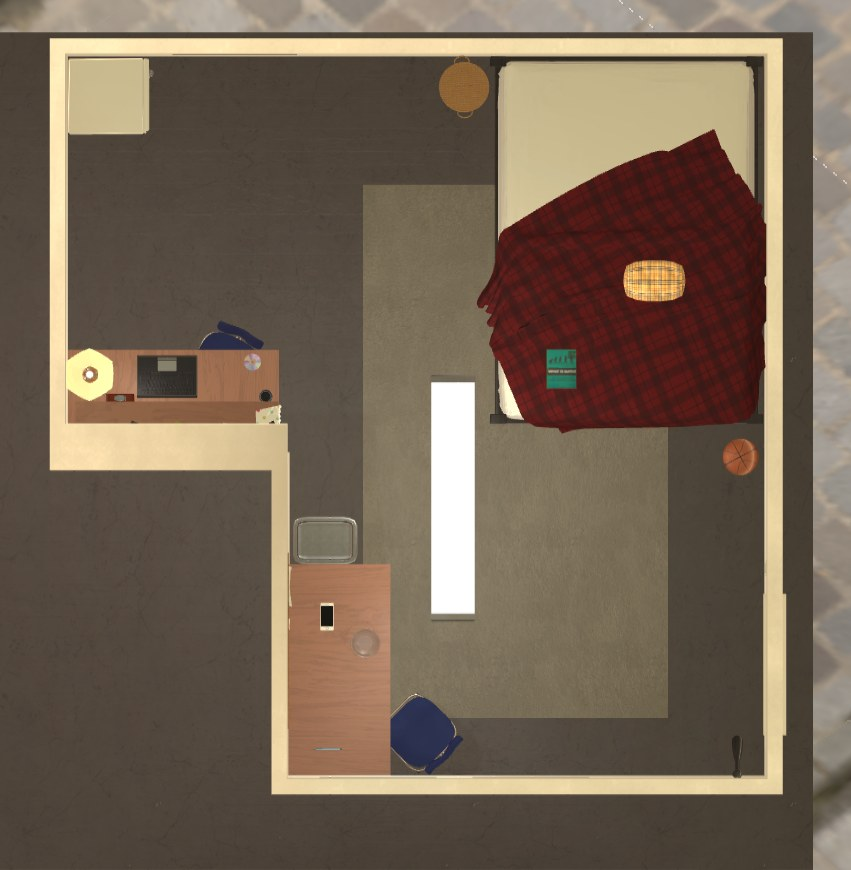
\includegraphics[width=6.242cm]{figures/cases/task0_map.jpg}};
\draw[black!35, line width=0.4pt] (8.758,0.000) rectangle ++(6.242,-6.381);
\fill[black, opacity=0.22] (10.861,-2.189) -- ++(-135:1.1) arc (-135:-45:1.1) -- cycle;
\fill[black] (10.861,-2.189) circle (0.08);
\draw[white, line width=3.4pt, opacity=0.85] (9.917,-3.289) -- (11.191,-4.899);
\draw[path] (9.917,-3.289) -- (11.191,-4.899);
\draw[lead=dimA] (9.792,-3.132) -- (10.845,-3.485);
\fill[dimA] (9.792,-3.132) circle (0.06);
\node[lblkey=dimA] at (10.845,-3.485) {shelf: the mug is here};
\draw[lead=liftpositive] (11.347,-5.095) -- (11.347,-4.595);
\fill[liftpositive] (11.347,-5.095) circle (0.06);
\node[lblkey=liftpositive] at (11.347,-4.595) {desk: put it here};
\draw[lead=black!55] (13.353,-1.719) -- (13.353,-1.219);
\fill[black!55] (13.353,-1.719) circle (0.06);
\node[lbl=black!45] at (13.353,-1.219) {bed};
\draw[lead=black!55] (10.211,-2.842) -- (10.211,-2.342);
\fill[black!55] (10.211,-2.842) circle (0.06);
\node[lbl=black!45] at (10.211,-2.342) {desk};
\draw[lead=black!55] (9.659,-2.774) -- (10.559,-2.965);
\fill[black!55] (9.659,-2.774) circle (0.06);
\node[lbl=black!45] at (10.559,-2.965) {drawers};
\draw[lead=black!55] (11.415,-4.542) -- (11.415,-4.042);
\fill[black!55] (11.415,-4.542) circle (0.06);
\node[lbl=black!45] at (11.415,-4.042) {drawers};
\draw[lead=black!55] (11.143,-3.966) -- (9.953,-3.966);
\fill[black!55] (11.143,-3.966) circle (0.06);
\node[lbl=black!45] at (9.953,-3.966) {garbagecan};
\draw[lead=black!55] (12.162,-0.638) -- (11.375,-0.285);
\fill[black!55] (12.162,-0.638) circle (0.06);
\node[lbl=black!45] at (11.375,-0.285) {laundryhamper};
\draw[lead=black!55] (9.536,-0.706) -- (9.296,-0.244);
\fill[black!55] (9.536,-0.706) circle (0.06);
\node[lbl=black!45] at (9.296,-0.244) {safe};
\draw[lead=black!55] (10.236,-3.132) -- (9.337,-2.941);
\fill[black!55] (10.236,-3.132) circle (0.06);
\node[lbl=black!45] at (9.337,-2.941) {shelves};
\node[imgcap] at (4.254,-6.421) {first-person view inside the room};
\node[imgcap] at (11.879,-6.421) {the room from above; cone: the left view; arrow: the expert's route};
\node[anchor=west, font=\sffamily\bfseries\footnotesize, text=black!70] at (0,-7.181) {Expert solution (4 steps):};
\node[chip, anchor=west] (s0) at (3.900,-7.181) {go to shelf};
\node[chip, anchor=west] (s1) at (6.162,-7.181) {take mug from shelf};
\draw[flow] (s0.east) -- (s1.west);
\node[chip, anchor=west] (s2) at (9.560,-7.181) {go to desk};
\draw[flow] (s1.east) -- (s2.west);
\node[chip, anchor=west] (s3) at (11.680,-7.181) {move mug to desk};
\draw[flow] (s2.east) -- (s3.west);
\node[ptitle] at (0.000,-7.981) {(b) What happened: \texttt{GPT-4o-mini}, seed 0};
\node[lab] at (1.650,-8.581) {expert};
\fill[black!30, rounded corners=1pt] (1.750,-8.431) rectangle ++(0.800,-0.3);
\node[txt] at (2.630,-8.581) {4};
\node[lab] at (1.650,-9.041) {no memory};
\fill[phaseA!35, rounded corners=1pt] (1.750,-8.891) rectangle ++(3.800,-0.3);
\node[txt] at (5.630,-9.041) {19, solved};
\node[lab] at (1.650,-9.501) {memory};
\fill[salmon!60, rounded corners=1pt] (1.750,-9.351) rectangle ++(1.200,-0.3);
\node[txt] at (3.030,-9.501) {6, solved};
\draw[densely dashed, black!40] (7.750,-8.331) -- (7.750,-9.761);
\node[font=\sffamily\scriptsize, text=black!50, anchor=north] at (7.750,-9.761) {30-step limit};
\node[txt] at (10.600,-8.581) {prompt tokens: 40,783 $\rightarrow$ 17,850};
\node[txt] at (10.600,-9.001) {effect over 3 demo pairs:};
\node[txt] at (10.600,-9.421) {\quad GPT $0.000$, Qwen $-0.333$};
\end{scope}
\end{tikzpicture}
